\section{Template Generation and Matching\label{template-generation}}

\subsection{Finger Knuckle Template Generation\label{fk-template}}

\begin{figure*}
    \centering
    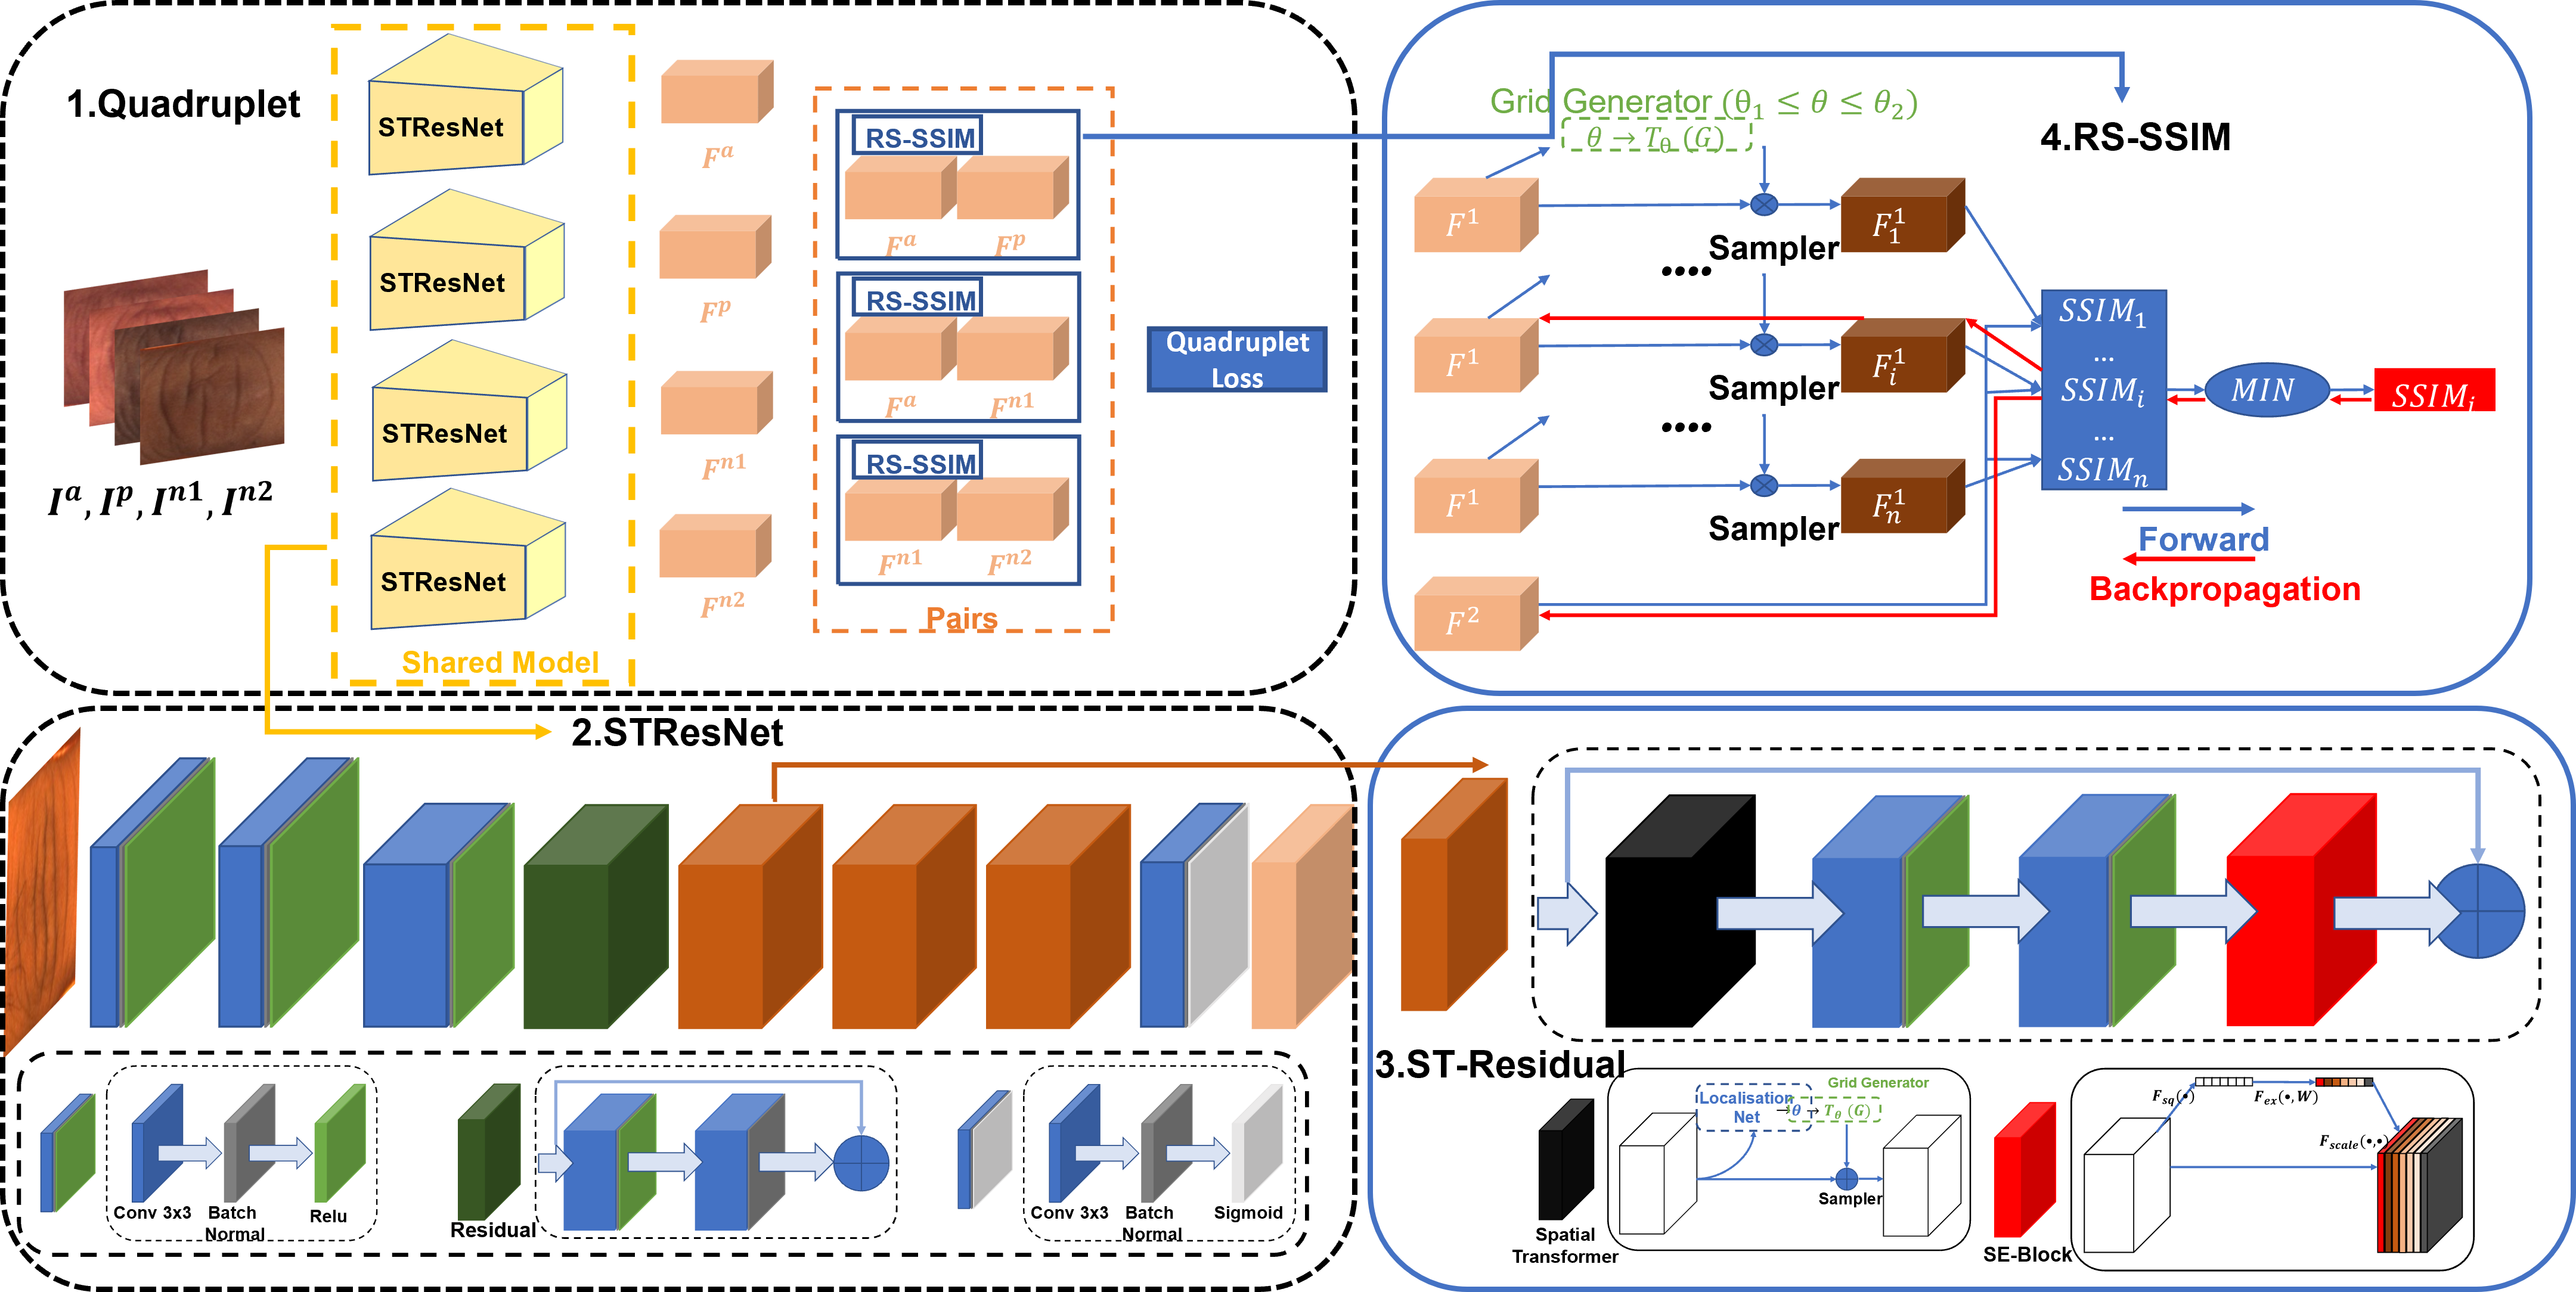
\includegraphics[width=6.5in]{Figures/framework/ST-Residual/Framework.png}
    \caption{We have proposal a new finger knuckle recognition framework with quadruplet. 1. Quadruplet: We trained our model with the quadruplet loss \cite{chen2017beyond} for decreasing inter-class variance and increasing intra-class variance. 2. FKMBConv: The new model use four repeated MBConv block \cite{tan2021efficientnetv2} for enhancing channel information, and it output a 64 channels feature maps. 3. ST-Residual: It consists of a
     4. RS-SSIM: Meanwhile, we introduce a new loss function based on the SSIM index for enhance the FKMBConv rotation and translation invariance ability by rotating and shifting output feature maps.}
    \label{framework}
\end{figure*}

Each of the segmented and normalized finger-knuckle images are subjected to the feature extraction to generate respective templates for the matching. There are a range of spatial domain \cite{sricharan2006knuckle}, \cite{kumar2009personal}, \cite{zhang2010online}, \cite{zhu2010multimodal}, \cite{zheng20163d}, \cite{kumar2016personal} and spectral domain \cite{aoyama2011finger}, \cite{kumar2015recovering} methods investigated in the literature to match finger knuckle patterns. Among these methods spatial-domain methods are quite attractive as they are computationally simpler and have shown to offer state-of-the-art results. \sout{We employed the local feature descriptor based approach introduced in \cite{zheng20163d}, \cite{kumar2016personal} to generate finger knuckle templates as this approach is computationally attractive, accurate and generates smallest finger-knuckle templates (one-bit-per-pixel) that can be more conveniently stored along with the fingerprint-templates for the real applications.} \textcolor{red}{At the same field, deep learning model have achieved the state-of-the-art performance, such as the RFN \cite{liu2020contactless}, FKNet \cite{cheng2020deep}, and so on.}

\textcolor{red}{Comparing to these above non-deep learning and deep learning, we introduce a new CNN architecture based on the EfficientNetV2-S backbone \cite{tan2021efficientnetv2} which have outperformed the state-of-the-art classifier neural network on the ImageNet ILSVR2012 and ImageNet21k dataset \cite{russakovsky2015imagenet}. We just want to extract the texture features from finger knuckle images instead of high level feature maps. Therefore, we use the FKMBConv model, in the Fig. \ref{framework}, as the feature extract backbone. After extracting the feature maps, we can use MSE, PSNR and SSIM \cite{wang2004image} to calculate the similarity score between two feature maps. As for the MSE and PSNR, they calculate the absolute difference between two images. However, SSIM \cite{wang2004image} can get the structural similarity which is very robust when compare two texture feature maps. It can use sliding window approach to get the local matching score and get the mean value of all local matching score between two images, which is very fit on matching two texture feature maps.} 

\textcolor{red}{As we mentioned in the Section \ref{motivation-contribution}, the CNN model does not have the rotational and translational invariance capability, nor dose SSIM. Therefore, we also proposal a new loss based on the SSIM, called RS-SSIM in the Fig. \ref{framework}, and it can rotate and shift feature maps in a \textit{predefined} range $\theta_1 \leq \theta \leq \theta_2$ by grid generator and sampler followed the reference \cite{jaderberg2015spatial} for getting more robust similarity scores which can reduce the inter-class variance. Among these rotated and shifted templates, we will get the minimal value $SSIM_i$ form the $F_i^1$, then the backpropagation will along the $F_i^1$ path to update the model learnable weights. In order to enable the whole network FKMBConv to update the weights in training process, we implement a differentiable SSIM so that the network can be trained smoothly. Then we trained our proposal framework with the quadruplet architecture \cite{chen2017beyond} on the segmented middle finger knuckle of left hand. It is worthy to note that how to choose the quadruplet when we train our model. Each subject offers five samples, so that for the positive ($p$), we choose the one with the largest SSIM distance with the anchor ($a$) among the remaining four samples in the same subject data. We arbitrarily choose two other different subjects, and tow with the smallest gap with the anchor ($a$) as negative1 ($n1$) and negative2 ($n2$). We have presented our experiment results in the Section \ref{fk-performance}, and compare to the state-of-the-art finger knuckle recognition model on the Section \ref{discussion}.}


\subsection{Fingerprint Template Generation\label{fp-template}}

Among a range of methods introduced in the literature \cite{maltoni2009handbook} to match fingerprint images, minutiae-based methods are widely employed and therefore preferred. We considered a range of popular methods and implementations available in the references to generate fingerprint templates. Among various fingerprint matchers employed in the literature, NBIS (NIST Biometric Image Software) \cite{cappelli2010minutia} and minutiae cylinder code (MCC) \cite{watson2007user} are quite popular. We also considered a commercial off-the-shelf (COTS) matcher \cite{verifinger} which has shown quite accurate results in many references. Simultaneously acquired fingerprint images from the slap-fingerprint sensors are automatically segmented and employed to generate fingerprint templates. These templates are used to generate respective match scores that are consolidated for the user authentication. 

\subsection{Dynamic Score Consolidation\label{dynamic-score}}

The match scores generated from two independent pieces of evidences are consolidated to achieve a more reliable decision score for the user authentication. Biometrics literature \cite{maltoni2009handbook} provides extensive investigation on a range of methods to consolidate decisions from two pieces of evidences or features. Such consolidation from can be achieved at feature level, score level, or at the decision level. The score level combination is most widely used in the literature and is widely adapted \cite{jain2012biometric} in a range of biometrics system, largely due to its simplicity and the performance. The objective of our system is to serve as an add-on system on the top of existing or deployed slap-fingerprint system where the match scores are inherently available from the respective minutiae templates. Therefore, score level combination was preferred and adapted for the score consolidation in our system.  
\begin{algorithm}[h!]
    \renewcommand{\algorithmicrequire}{\textbf{Input:}}
    \renewcommand{\algorithmicensure}{\textbf{Output:}}
    \caption{Dynamic Match Score Consolidation}
    \begin{algorithmic}[1]
        \REQUIRE Match score $\bm{s_k, s_f, q_k, q_f}$ \\ 
        \ENSURE Consolidation score $\bm{s_c}$;\\
        \IF {$q_k = 0 $ and $0 < q_f \leq 1$}
            \STATE $s_c = s_f$
        \ENDIF
        \IF {$ 0 < q_k \leq 1$ and $q_f = 0$}
            \STATE $s_c = s_k$
        \ENDIF
        \IF {$q_k = 0$ and $q_f = 0$}
            \STATE $s_c = 0$
        \ELSE
            \STATE $s_c = w \times s_k + (1-w)*s_f$
        \ENDIF
        \RETURN $s_c$
    \end{algorithmic}
    \label{algorithm-2}
\end{algorithm}

Real biometric systems during their deployments are often presented with missing or degraded quality of biometric samples and therefore the score-level consolidation scheme should be adaptive to such inputs. Therefore, we developed a dynamic scheme to consolidate match scores from two simultaneously generated match scores from the fingerprint and the finger knuckle. Let the match score from fingerprint be represented by $s_f$ and the match score from the finger knuckle be represented by $s_k$. The confidence or the quality of input biometric image sample, as shown in Fig. \ref{block-diagram}, can be denoted as $q_k$ and $q_f$ respectively for the finger knuckle and fingerprint. \textcolor{red}{If we can not detect or segment the finger knuckle or fingerprint, we use the score 0 to represent it.} The consolidated match score $s_c$ is generated as shown in Algorithm \ref{algorithm-2}. The weight $w ( 0 \leq w \leq 1)$  represents weight and is fixed empirically for all the experimental results in this paper. This scheme ensures that in case of missing or low quality biometric images, the importance is automatically granted for the other biometric modality.  

